\documentclass{article}

\usepackage{listings}
\usepackage{xcolor}
\usepackage{graphicx}

\definecolor{codegreen}{rgb}{0,0.6,0}
\definecolor{codegray}{rgb}{0.5,0.5,0.5}
\definecolor{codepurple}{rgb}{0.58,0,0.82}
\definecolor{backcolour}{rgb}{0.95,0.95,0.92}

\lstdefinestyle{mystyle}{
    backgroundcolor=\color{backcolour},
    commentstyle=\color{codegreen},
    keywordstyle=\color{magenta},
    numberstyle=\tiny\color{codegray},
    stringstyle=\color{codepurple},
    basicstyle=\ttfamily\footnotesize,
    breaklines=true,
    keepspaces=true,
    numbers=left,
    numbersep=5pt,
    showspaces=false,
    showstringspaces=false,
    showtabs=false,
    tabsize=2
}

\lstset{style=mystyle}

\title{A TPTP Formalization of the Unified Foundational Ontology}
\author{
    Daniele Porelo,
    Jo\~ao Paulo A. Almeida,
    Giancarlo Guizzardi,\\
    Claudenir M. Fonseca,
    Tiago Prince Sales
}
\date{\today}

\begin{document}
\maketitle

\begin{abstract}
This document presents a formalization of the Unified Foundation Ontology (UFO) expressed in first-order logics through the TPTP syntax. This formalization is intended to support verification of UFO's theory through automated provers and consistency checkers.
\end{abstract}

\section{Introduction}

This document presents a formalization of the Unified Foundation Ontology (UFO) expressed in first-order logics through the TPTP syntax. This formalization is intended to support verification of UFO's theory through automated provers and consistency checkers.

\section{UFO's TPTP Specification}

\subsection{UFO Taxonomy}

% Thing Taxonomy

\begin{figure}[ht]
    \centering
    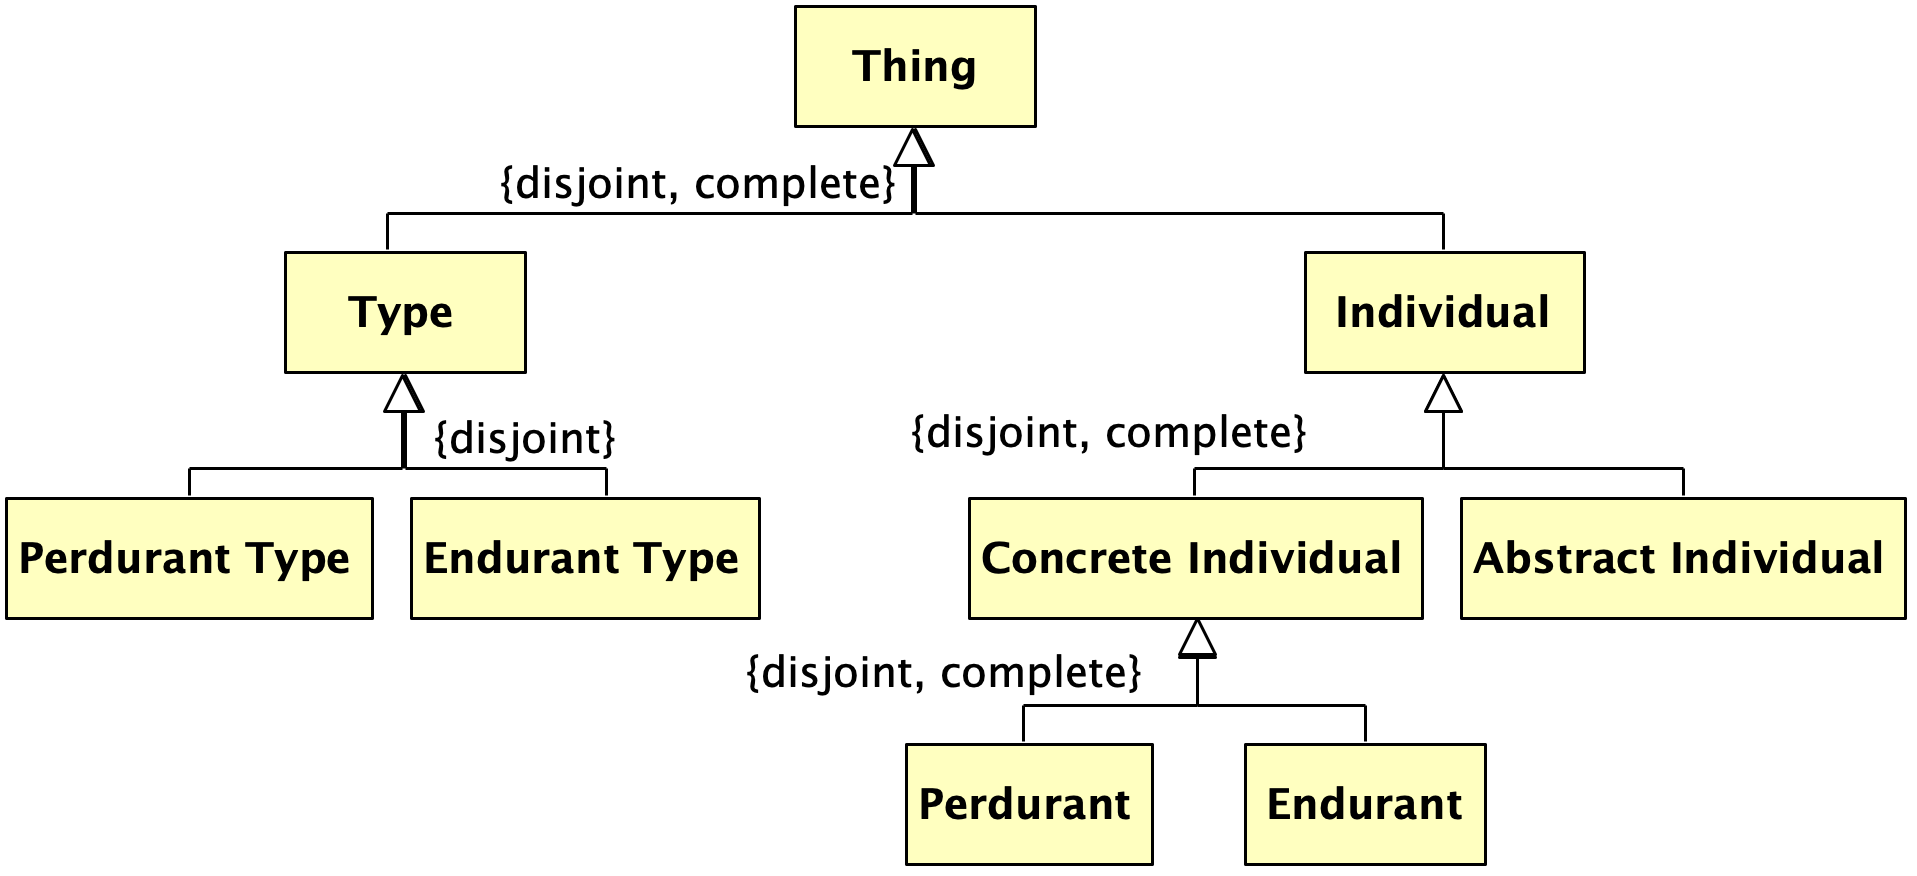
\includegraphics[width=0.8\textwidth]{diagrams/Thing_Diagram.png}
    \caption{Partial Taxonomy of UFO -- Thing.}
    \label{fig:ufo_taxonomy_thing}
\end{figure}

\lstinputlisting[firstline=4, lastline=48, firstnumber=4]{ufo_2021.tex}

% Abstract Individual Taxonomy

\begin{figure}[ht]
    \centering
    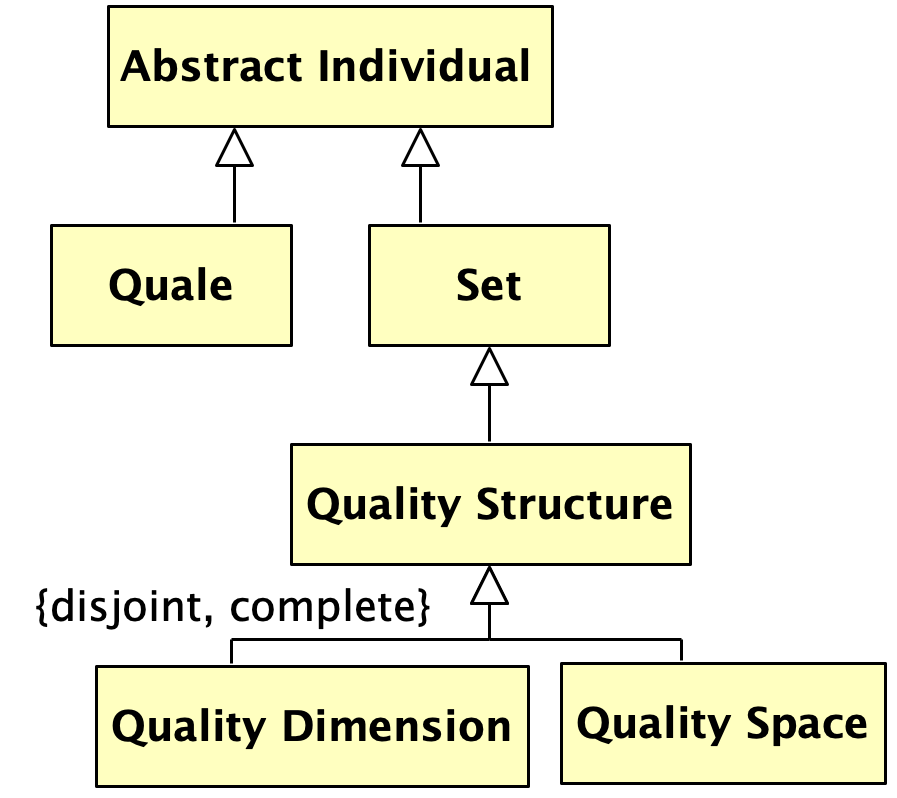
\includegraphics[width=0.4\textwidth]{diagrams/Abstract_Individual_Diagram.png}
    \caption{Partial Taxonomy of UFO -- Abstract Individual.}
    \label{fig:ufo_taxonomy_abstract_individual}
\end{figure}

\lstinputlisting[firstline=50, lastline=80, firstnumber=50]{ufo_2021.tex}

% Endurant Taxonomy

\begin{figure}[ht]
    \centering
    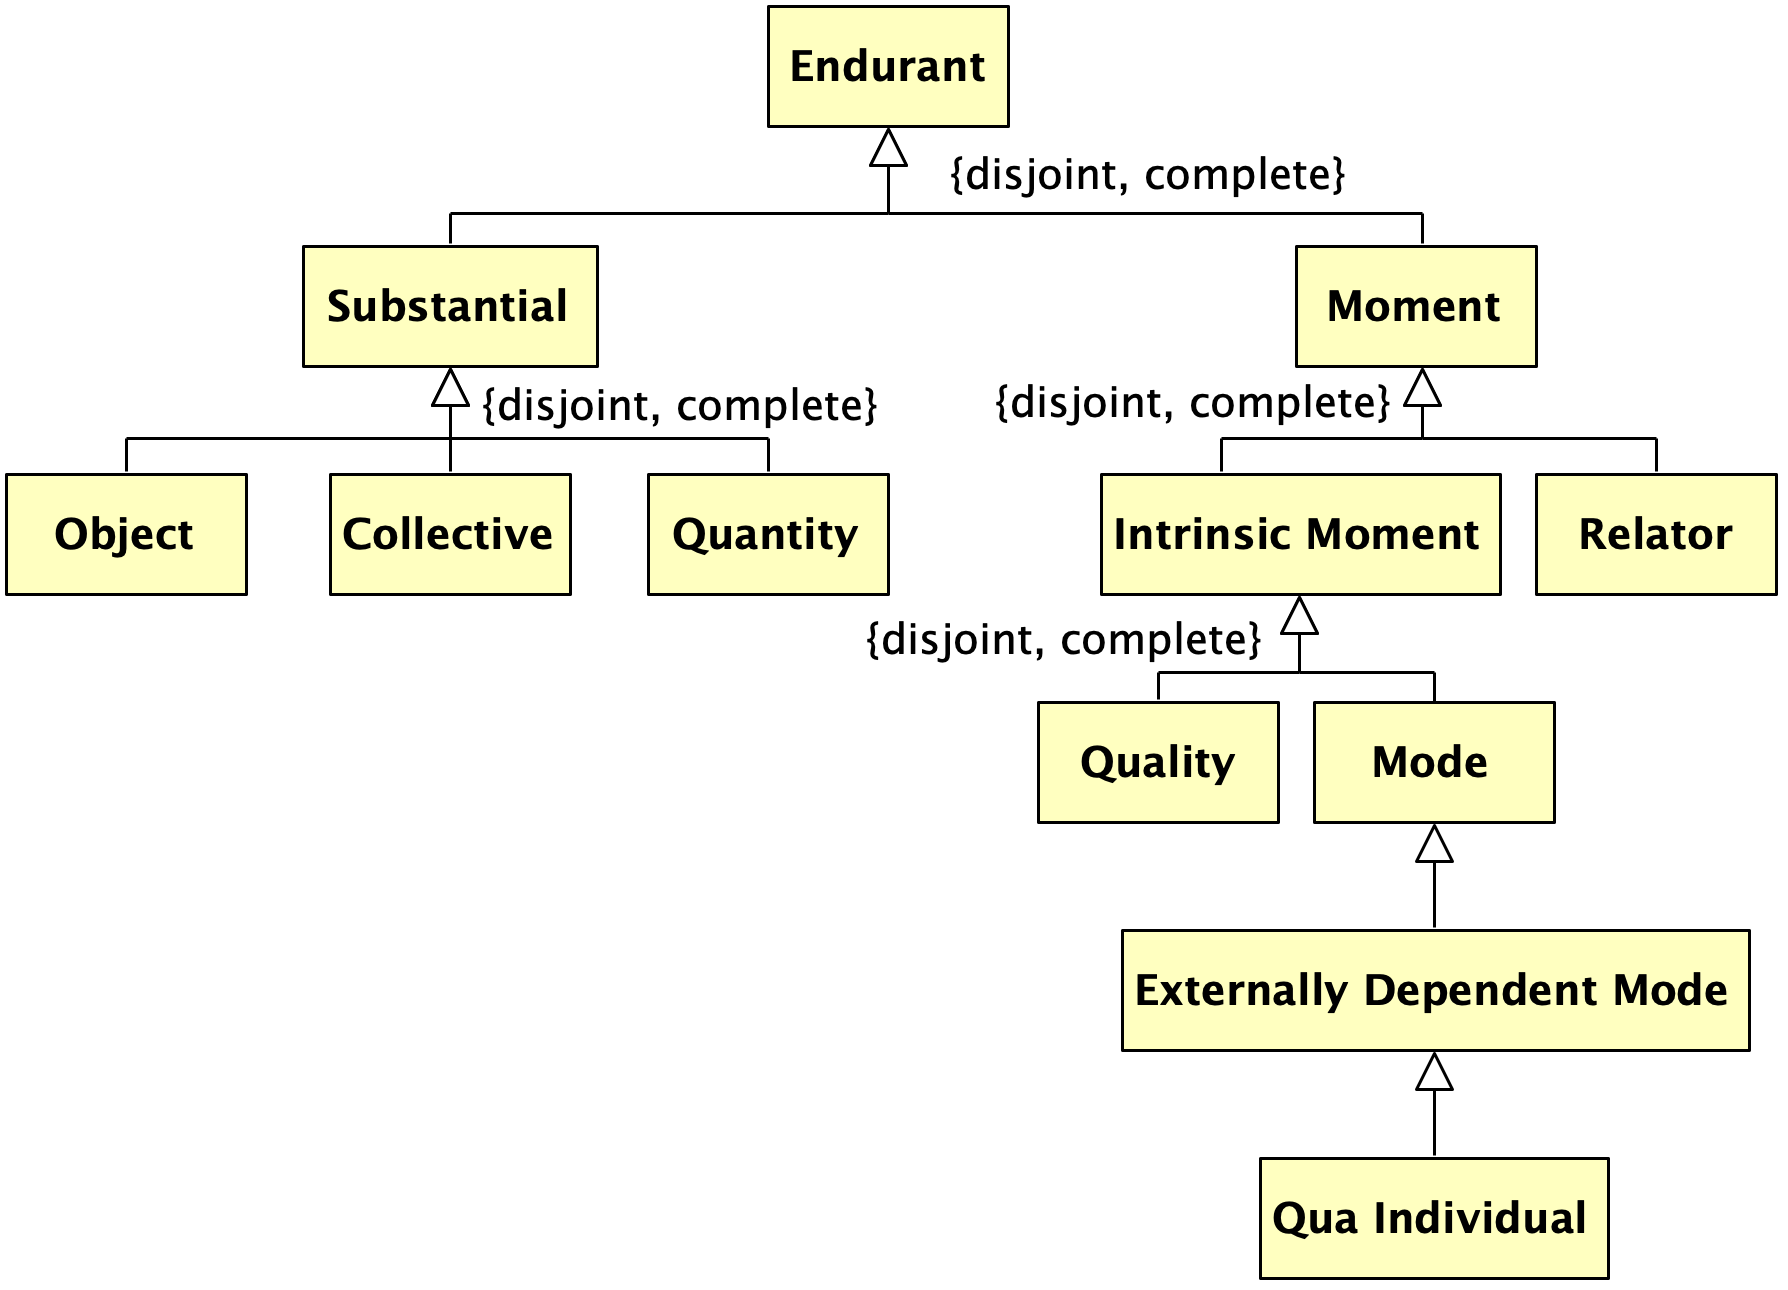
\includegraphics[width=0.8\textwidth]{diagrams/Endurant_Diagram.png}
    \caption{Partial Taxonomy of UFO -- Endurant.}
    \label{fig:ufo_taxonomy_endurant}
\end{figure}

\lstinputlisting[firstline=82, lastline=138, firstnumber=82]{ufo_2021.tex}

% Endurant Type Taxonomy of Ontological Natures

\begin{figure}[ht]
    \centering
    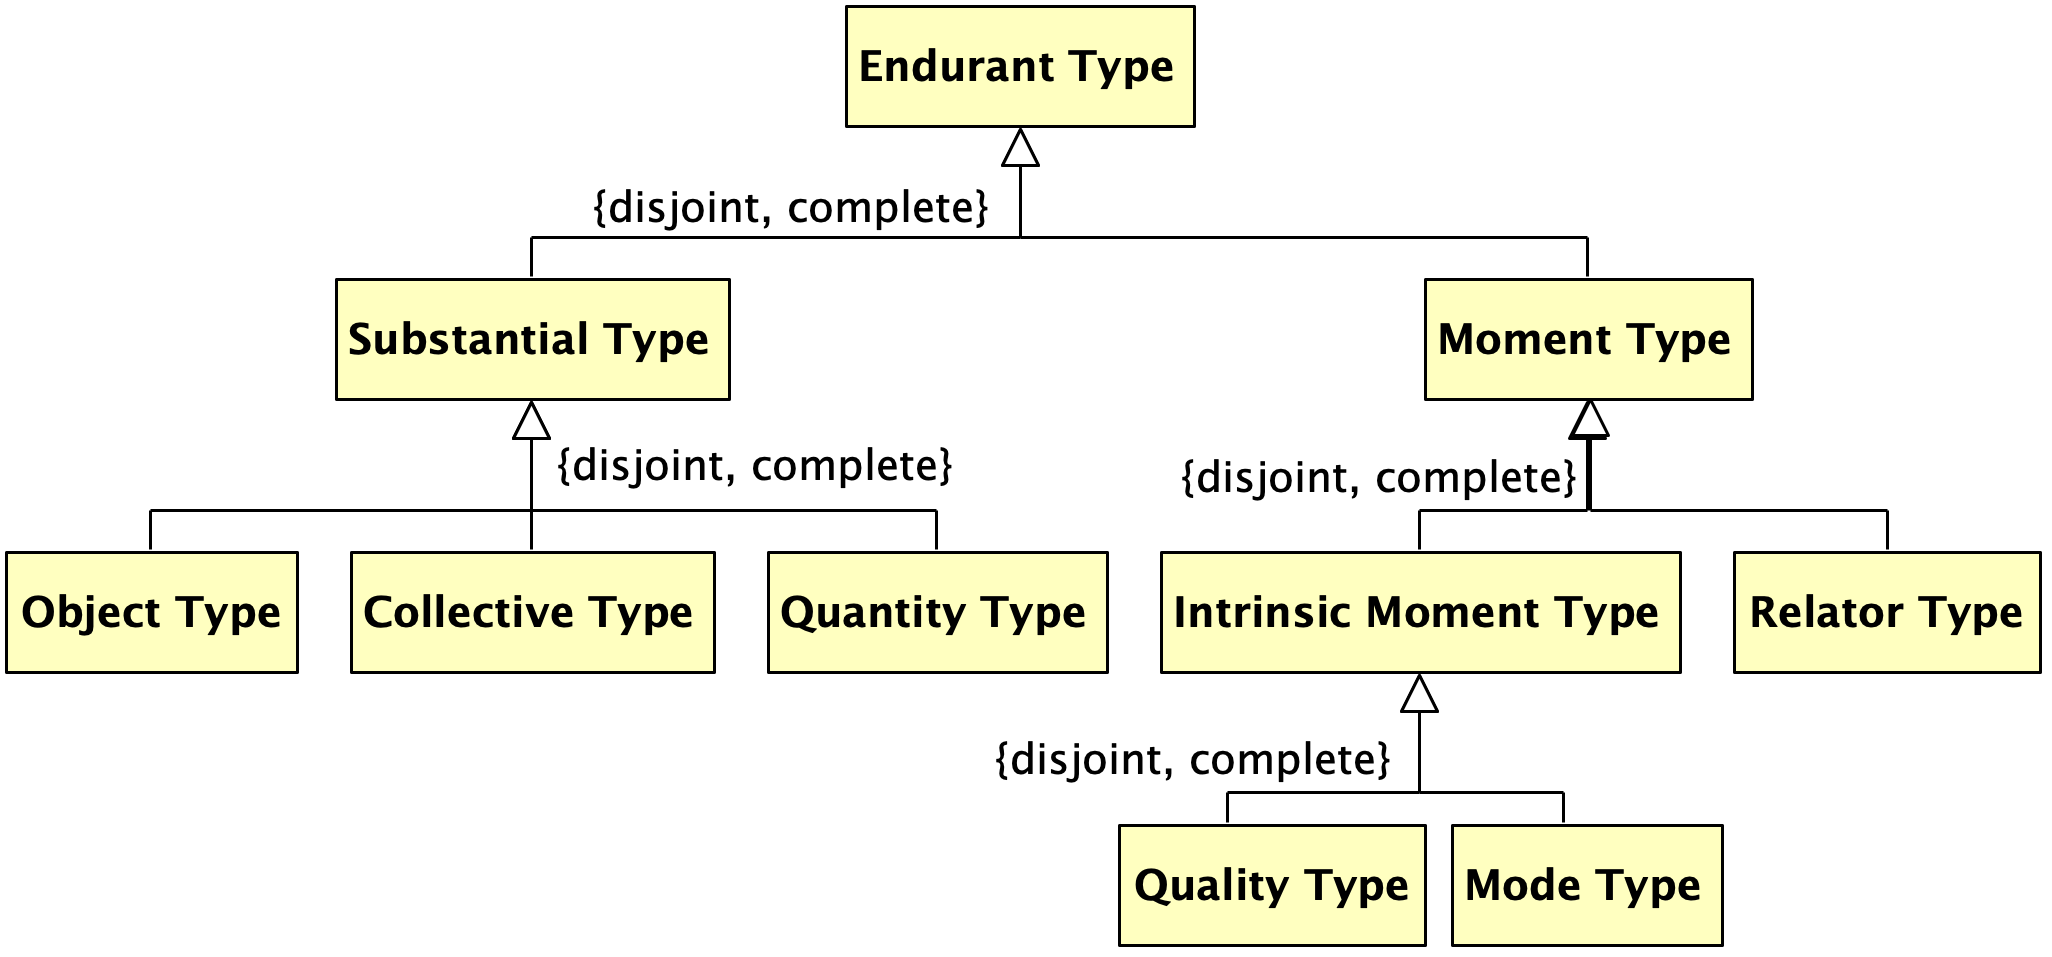
\includegraphics[width=0.9\textwidth]{diagrams/Endurant_Type_Natures_Diagram.png}
    \caption{Partial Taxonomy of UFO -- Endurant Types (by ontological nature).}
    \label{fig:ufo_taxonomy_endurant_types_natures}
\end{figure}

\lstinputlisting[firstline=140, lastline=184, firstnumber=140]{ufo_2021.tex}

% Endurant Type Taxonomy of Modal Properties of Types

\begin{figure}[ht]
    \centering
    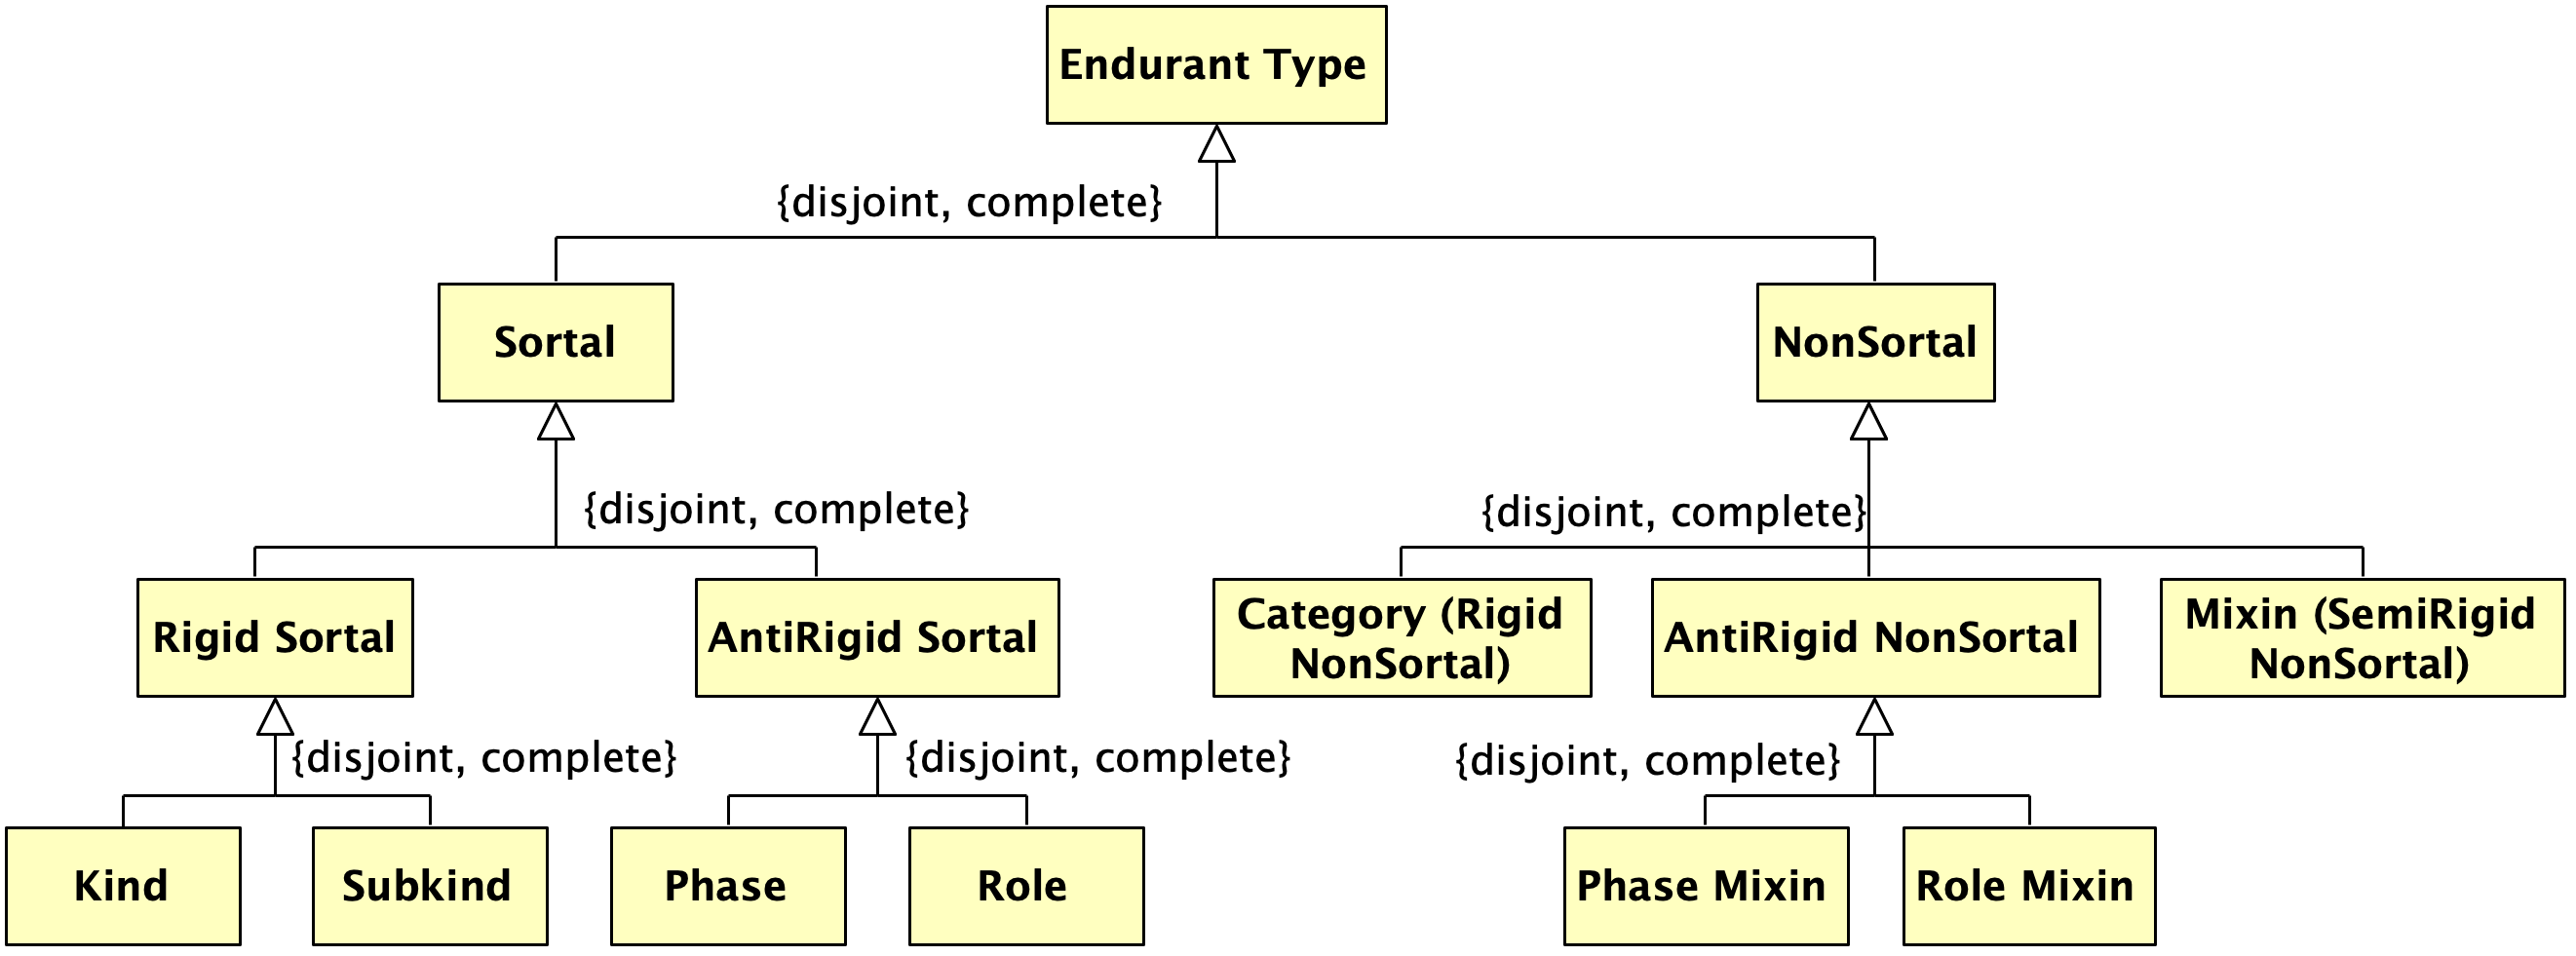
\includegraphics[width=\textwidth]{diagrams/Endurant_Type_Properties_Diagram.png}
    \caption{Partial Taxonomy of UFO -- Endurant Types (by modal properties of types).}
    \label{fig:ufo_taxonomy_endurant_types_properties}
\end{figure}

\lstinputlisting[firstline=186, lastline=262, firstnumber=186]{ufo_2021.tex}

% \bibliographystyle{abbrv}
% \bibliography{main}

\end{document}
% This is never printed